\section{Реконструкция треков частиц}

Трекинг в NA64 необходим для определения энергии и идентификации типа частиц
попадающих в электромагнитный калориметр и покидающих его
В постановке для изучения электромагнитных ливней вызванных электроном трекер
представляет собой двухплечевой спектрометр (систему мечения) составленный
из нескольких газовых детекторов, расположенных по оси пучка до и после магнита
перед электромагнитным калориметром (активной мишенью).
%с совокупным \emph{вкладом ??}.
Для мюонной постановки система мечения дополнительно оснащается станциями
BMS (beam momentum station). После калориметра устанавливается дополнительный
спектрометр представленный отклоняющим дипольным магнитом и дополнительными
станциями MM и ST с увеличенным аксептансом для идентификации частиц покидающих
ECAL.

В целом, высокое пространственное разрешение
и сравнительно слабая оснащённость детекторами (по две или три станции на плечо,
выбранная, с тем чтобы минимизировать ионизационные потери и рассеяние), а
так же применение детекторов с гальванически связанными каналами (MicroMega)
обуславливают особенности трекера~NA64:
\begin{enumerate}
    \item Низкая заселённость за исключением второго спектрометра в мюонной
    постановке. В постановке с электронным или адронным пучком среднее
    число треков на событие -- $1{,}4$.
    \item Линейная протяжённость в десятки метров при сравнительно малой площади
    чувствительной поверхности детекторов в сотню $\text{см}^2$.
    \item Присутствие ложных срабатываний в MicroMega из-за гальванического
    соединения анодных полос (коммутации в одну сигнальную линию).
\end{enumerate}

С одной стороны эти особенности обуславливают существенные методические
ограничения: невозможность эффективно использовать гало пучка для выравнивания,
и невозможность эффективно покрыть трекер в голове канала расфокусированным пучком
для выравнивания и изучения эффективности трекера.

С другой стороны, при сравнительно высоком пространственном разрешении
трекера, дающим энергетическое разрешение не более $1~\text{ГэВ}$,
и сам трекинг, и геометрическое выравнивание детекторов на его основе
вносят не столь существенный вклад в систематическую ошибку эксперимента.

\subsection{Реконструкция кластеров микроструктурных детекторов}

Оцифрованный сигнал с микроструктурных детекторов GEM и MicroMega представляет
собой кортеж из трёх чисел отвечающих измерениям амплитуды напряжения на переднем
фронте токового импульса соответствующего стрипа (металлической полоски на считывающей
поверхности детектора), как показано на рисунке~\ref{fig:apv-pulse-sampling}.

\begin{figure}
    \centering
    \includegraphics[width=0.45\linewidth]{images//illustrative/mm-amps.png}
    \caption{Сэмплирование переднего фронта сигнала с одного канала
    микроструктурного детектора~\cite{na64-BANERJEE201872}}
    \label{fig:apv-pulse-sampling}
\end{figure}

В рабочем режиме детектора средняя точка отвечает критерию постоянной
доле~(\emph{constant fraction}) и её относительное временное смещение не зависит от
амплитуды. Поскольку у элементов входных каскадов считывающей электроники присутствует
разброс параметров, вывод детектора в рабочий режим требует
подстройки фазы синхронизирующего импульса~\acrshort{sadc}.

Затем строится гистограмма отношений амплитуд $r_{02}=A_0/A_2$ и $r_{12}=A_1/A_2$,
пример которой приведён на рисунке~\ref{fig:banana-histogram}. Калибровка 
заключается в выборе дискриминирующего условия на отношение амплитуд на основе такого
распределения, выражающееся в параметризованном неравенстве (обычно, включающее
полигональную фигуру, полиномы, сплайны или кривые Безье) отсекающим паразитные
амплитуды в пределах выбранного доверительного интервала.

\begin{figure}
    \centering
    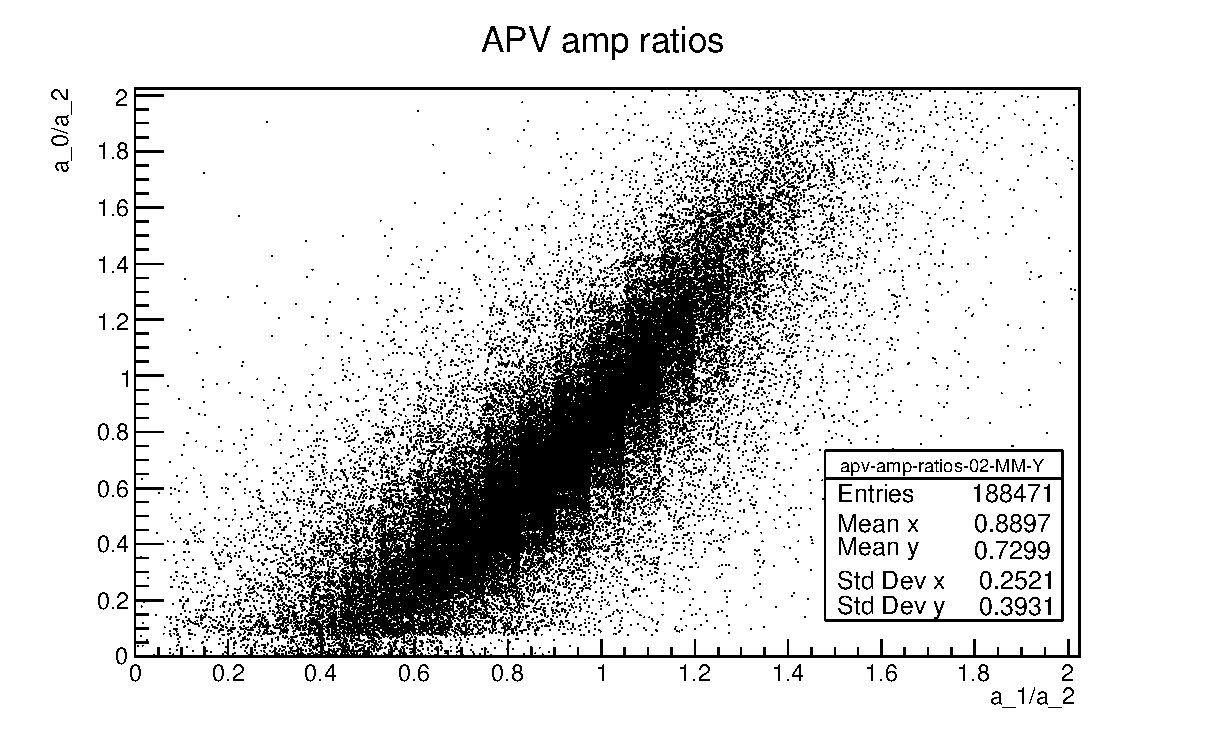
\includegraphics[width=0.45\linewidth]{images/illustrative/banana-example.eps}
    \caption{Пример распределения отношения амплитуд $r_{02}$ и $r_{12}$ переднего
    фронта сигнала микроструктурного детектора}
    \label{fig:banana-histogram}
\end{figure}

\subsection{Реконструкция измерений от тонкостенных трубок}

%Станции тонкостенных газоразрядных трубок предоставляют информацию
%о времени развития электронной лавины $t'$ в рабочем объёме конкретной
%трубки относительно времени срабатывания триггера. В $t'$ включено
%время пролёта частицы до трубки $\delta t$, которое для большинства
%релятивистских частиц (мюонов и электронов) принимается постоянным.
%Так, например, времяпролётная разница на дистанции в десять метров
%для электронов в $1~\text{ГэВ}$ и $100~\text{ГэВ}$ составляет
%менее $1~\text{пс}$, для мюонов -- менее $200~\text{пс}$, в то время
%как характерное время дрейфа лавины в трубке обычно составляет десятки
%наносекунд -- $20~\text{нс}$ для трубок диаметром $2~\text{мм}$
%и $50~\text{нс}$ для трубок $6~\text{мм}$. При принципиально-достижимом
%координатном разрешении в детекторах такого типа в $200~\text{мкм}$
%эта разница во временах для лептонов высоких энергий несущественна.
Станции тонкостенных газоразрядных трубок регистрируют время развития
электронной лавины $t'$ в рабочем объёме каждой трубки относительно
сигнала триггера. В это время включено также запаздывание
частицы $\delta t$, которое для большинства релятивистских частиц
практически постоянно. Так, например, различие
во времени пролёта на расстоянии десяти метров между электронами с
энергией $1~\text{ГэВ}$ и $100~\text{ГэВ}$ составляет менее $1~\text{пс}$,
а для мюонов~-- менее $200~\text{пс}$, тогда как характерное время
дрейфа лавины в трубке находится на уровне десятков наносекунд:
около $20~\text{нс}$ для трубок диаметром $2~\text{мм}$ и порядка
$50~\text{нс}$ для трубок диаметром $6~\text{мм}$. При достижимом
координатном разрешении таких детекторов порядка $200~\text{мкм}$
указанные различия во времени пролёта для лептонов высоких энергий
не имеют существенного значения.

%По этой причине $t'$ определяется главным образом временем $T$ дрейфа
%электронной лавины в разрядном промежутке трубки от ближайшей точки
%ионизации до катодной проволоки с расстоянием $R$, которое в свою очередь
%в наибольшей степени зависит от давления и плотности газовой смеси.
Таким образом, величина $t'$ определяется главным образом временем $T$
дрейфа электронов в разрядном промежутке трубки от ближайшей точки
ионизации до катодной проволоки.

%Таким образом зависимость $R(T)$, хотя и имеет нелинейный характер,
%хорошо поддаётся аппроксимации различными аналитическими моделями.
%Параметры такой модели и составляют необходимую калибровочную
%информацию применяемую при определении радиуса
%изохроной цилиндрической поверхности задаваемой временем срабатывания~$T$.
Функция $R(T)$ имеет нелинейный характер, однако хорошо аппроксимируется
различными аналитическими моделями. Параметры такой аппроксимации и
составляют необходимую калибровочную информацию, используемую при
определении радиуса изохронной цилиндрической поверхности, соответствующей
данному времени срабатывания~$T$.

На рисунке~\ref{fig:straws-rt} изображена гистограмма полученная для
трубки диаметром $6~\text{мм}$, находящейся
позади адронного калориметра с наложенными поверх гистограмм аппроксимациями
зависимости $R(T)$.
%\begin{figure}[ht]
%    \centering
%    \includegraphics[width=0.95\linewidth]{images/illustrative/ST-RT.jpg}
%    \caption{Распределение $R(T)$ для нескольких трубок станции ST
%    диаметром $6~\text{мм}$ (ось времени инверирована)}
%    \label{fig:straws-rt}
%\end{figure}
\begin{figure}
    \centering
    \includegraphics[width=0.33\linewidth]{images//illustrative/ST-RT-single-mono.png}
    \caption{Распределение $R(T)$ для нескольких трубок станции ST
    диаметром $6~\text{мм}$, $R$ в мм, время в относительных единицах, ось времени инверирована}
    \label{fig:straws-rt}
\end{figure}
Большое количество срабатываний отстоящих от основной линии обусловлено
высоким фоном от вторичных частиц.

%Хотя определение радиуса изохронной поверхности таким образом представляет
%собой простую задачу (реализуемую при помощи единственного обработчика,
%применяющего калибровочные данные), последующее использование этой
%информации в
%алгоритмах трекинга требует привлечения нетривиальных
%алгоритмов либо на этапе предварительного поиска треков, либо
%в процессе подгонки параметров модели трека. В простейшем случае, проводят
%плоскость через оси трубок в одной координатной проекции, и отмечают
%линии пересечения изохронной поверхности с этой плоскостью. Получившиеся
%линии таким образом являются геометрическим местом возможного пересечения
%траектории частицы с плоскостью детектора с фиксированным разрешением.
%Поскольку для одной трубки таких линий образуется две, одной трубки
%недостаточно для определения координат частиц в одной проекции.
Хотя определение радиуса изохронной поверхности в таком подходе
представляет собой относительно простую задачу (реализуемую с помощью
единственного обработчика, использующего калибровочные данные),
дальнейшее применение этой информации в алгоритмах трекинга требует
привлечения более сложных методов -- как на этапе предварительного
поиска треков, так и при подгонке параметров модели трека. 

В простейшем случае через оси трубок в одной координатной проекции
проводится плоскость, и фиксируются линии пересечения изохронной
поверхности с этой плоскостью. Эти линии образуют геометрическое
место возможных точек пересечения траектории частицы с плоскостью
детектора при данном временном разрешении. Поскольку для одной трубки
возникают две такие линии, её информации недостаточно для определения
координаты частицы в одной проекции. Тем не менее, рассматривая показания
трековых детекторов в совокупности зачастую удаётся разрешить
возникающие неоднозначности. На рисунке~\ref{fig:evdisplay-new}
показана проекция пространственных примитивов изображающих
чувствительные объёмы детекторов MicroMega и станции трубок
совместно с допустимыми пределами разрешений (изображены
шириной $5\sigma$).

\begin{figure}[ht]
    \centering
    \includegraphics[width=0.5\linewidth]{images//illustrative/ST-evdisp-mono.png}
    \caption{Реконструкция треков по показаниям MicroMega (повёрнуты на $45^{\circ}$)
    со станициями тонкостенных разрядных трубок с изображением
    координатных разрешений и гипотезы трека с ковариационными конусами}
    \label{fig:evdisplay-new}
\end{figure}

%\begin{figure}
%    \centering
%    \includegraphics[width=0.5\linewidth]{images/illustrative/ST-evdisp.jpg}
%    \caption{Реконструкция треков в SPA}
%    \label{fig:evdisplay-new}
%\end{figure}

Возможны и более сложные алгоритмы реконструкции, учитывающие
трёхмерную структуру изохронных поверхностей в рамках одной станции
тонкостенных трубок~\cite{straws-peshekhonov2015}.

\subsection{Поиск треков}

%Задача предварительного поиска треков (англ. \emph{pattern recognition})
%состоит в выборе таких комбинаций пространственных объектов соответствующих
%отдельным измерениям, которые с заданной
%степенью правдоподобия могут образовывать трек частицы.
Задача предварительного поиска треков (англ. \emph{pattern recognition})
заключается в отборе таких комбинаций пространственных объектов,
соответствующих отдельным измерениям детектора, которые с заданной
степенью правдоподобия могут образовывать трек частицы.

%Среди множества существующих на сегодняшний день алгоритмов предварительного
%поиска треков~\cite{MankelTracking}, интерес представляет алгоритм
%CATS~\cite{catsc-JINR, catsc-discrete, catsc-nim, catsc-disto},
%(англ. \emph{cellular automata track search} -- в разное время авторы
%публиковали его формализацию в терминах <<эластичных>> нейронных сетей,
%и клеточных автоматов), который допускает весьма общую
%формулировку в силу независимости по отношению к конкретным
%геометрическим свойствам входных данных.
Среди многочисленных алгоритмов предварительного поиска~\cite{MankelTracking}
интерес представляет метод CATS
(англ. \emph{cellular automata track search})~\cite{catsc-JINR, catsc-discrete, catsc-nim, catsc-disto}.
В различных публикациях он излагался как в терминах <<эластичных>>
нейронных сетей, так и в формализме клеточных автоматов. 
Алгоритм допускает весьма общую формулировку в силу независимости по
отношению к конкретным геометрическим свойствам входных данных.

Формально задача, решаемая алгоритмом, может быть представлена следующим образом.
Пусть имеется
набор объектов $h_1,h_2, ...h_n$. Требуется найти такие
последовательности $(h_i,h_j,...h_m)$, для которых любая тройка
элементов $(h_{i-1},h_{i},h_{i+1})$ удовлетворяет заданному
условию $F(h_{i-1},h_{i},h_{i+1})=1$.
Основная идея состоит в эффективной стратегии обхода
объектов, позволяющей в большинстве случаев избежать прямого перебора
всех возможных комбинаций. Для этого алгоритм опирается на топологическую информацию
о <<слоях>> связанных с каждым объектом $h_i$. Каждому объекту сопоставляется
внутреннее состояние, обновляемых за конечно число итераций согласно
определённому правилу.

Пример работы алгоритма приведен на рисунке~\ref{fig:catsc-nim},
где приведены начальное и конечное состояния графа для синтетического набора
данных. Слои отмечены пунктирными
линиями, объекты $h$ (hits) изображены кругами, рёбра между парами
объектов -- сплошными линиями, а увеличенная толщина линии указывает
на больший вес соответствующей пары.

\begin{figure}
    \centering
    \includegraphics[width=0.45\linewidth]{images//illustrative/catsc-quote-it1.png}
    \includegraphics[width=0.45\linewidth]{images//illustrative/catsc-quote-it6.png}
    \caption{Начальное и конечное состояние графа связности после шести итераций алгоритма CATS~\cite{catsc-nim}}
    \label{fig:catsc-nim}
\end{figure}

В простейшем случае, в качестве объектов $h$ выбираются пространственные
точки, а условием $F$ является условие на максимальный пространственный
между ними $F(h_{i-1},h_{i},h_{i+1}): \angle(h_{i-1}h_i) (h_i h_{i+1}) < \theta_{th}$.

В результате время работы алгоритма оказывается существенно ниже
прямого перебора, в худшем случае ($\theta_{th} =\pi$) имея
сложность $\mathcal{O}(Ln^3)$, где $L$ -- число слоёв,
и $n$ -- число объектов $h$. Практически, сложность регулируется
функцией-фильтром, и при трудоёмкости фильтра~$\mathcal{O}(1)$ алгоритм
имеет сложность $\mathcal{O}(Ln^2)$. Наивный перебор троек $h$
с фильтрующей функцией дающей в среднем $d$ объектов в следующем слое
имеет сложность $\mathcal{O}(n^3 d^{L-3})$. Без фильтрующей функции
максимальная сложность возрастает экспоненциально $\mathcal{O}(n^L)$,
однако главное преимущество CATS перед наивной реализацией состоит
в устранении экспоненциального роста памяти, необходимой для хранения
гипотез. Алгоритм сводит задачу к итеративному линейному обходу
двунаправленного графа.

В оригинальных работах~\cite{catsc-JINR, catsc-discrete, catsc-nim, catsc-disto}
$h_i$ рассматриваются как пространственные точки $h_i:=\vec{r}_i$, или кортежи из
координат и времени $h_i:=(\vec{r}_i,t_i)$, в то время как алгоритм сам по себе
не подразумевает какого-то конкретного набора свойств, а требует
только того, чтобы определена функция $F:h_{1,2,3} \rightarrow \{0,1\}$.

Дополнением оригинального алгоритма является определение весовых
коэффициентов возвращаемых функцией-фильтром, то есть в более общем
случае $F: F(h_{1,2,3}) =w_j, ~w_j \in \mathbb{R_1}$. Кроме того, после
конструирования графа связности стратегия извлечения гипотез (обхода точек)
может допускать различные формы, что в оригинальных работах не
рассматривается. В частности, в случае когда одна и более гипотез $T_p, T_q$
претендуют на один и тот же сегмент $T_p \cap T_q = (h_i, h_j)$ выбор в пользу
той или иной гипотезы целесообразно бывает разрешать руководствуясь различными
критериями. Стратегии обхода результирующего графа реализованы в виде
программных модулей.

\subsection{Аппроксимация треков}

Классическая задача восстановления трека по измеренным
координатам в NA64 решалась различными методами.
Наиболее недавним является применение фильтра Калмана~\cite{kalman-1960},
реализованного библиотекой GenFit2~\cite{Genfit2_Rauch_2015}
в различных редакциях и с дополнениями оригинального алгоритма, из которых
наибольший практический интерес в контексте NA64
представляют
DAF (англ. \emph{deterministing annealing filter}~\cite{daf-track-fitting})
и KRF
(англ. \emph{Kalman filter with reference track}~\cite{krf-kalman-w-reference-track}).

Для подгонки параметров модели треков в условиях сложной геометрии
применяется KRF.
Его особенность по сравнению с оригинальным алгоритмом фильтра Калмана
состоит в том, что линеаризация уравнений переноса и измерений
выполняется не в малой окрестности предсказания, а
относительно заранее заданной опорной траектории,
обновляемой затем в несколько итераций. Этот приём позволяет снизить
систематические искажения при аппроксимации трека в
неоднородном магнитном поле, с учётом эффектов множественного
рассеяния (например, при проведении трека через калориметр).
Использование данного метода оправданно в сочетании с алгоритмами
поиска треков, которые задают разумное начальное приближение
для опорной траектории -- таких, как CATS~\cite{catsc-nim}.

DAF решает иную задачу: выбор согласованного подмножества
измерений в условиях неоднозначностей и загрязнений. В
его основе лежит назначение весов отдельным хитам с
последующей процедурой итеративного обновления весов. Вначале все
измерения вносят вклад в $\chi^2$-функцию, затем веса асимптотически
сходятся к согласованной гипотезе. В пределе это приводит к отбору
хитов, принадлежащих правдоподобной гипотезе с эффективным
исключением ложных срабатываний.
